\paragraph{Contact avec frottement solide}

\begin{wrapfigure}[10]{r}{0pt}
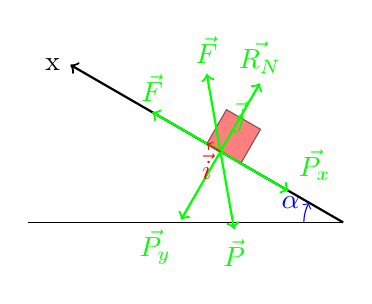
\begin{tikzpicture}
	\draw (0, 0) -- (-4, 0);
\draw[->, thick] (0, 0) -- (150:4) node [left] {x};
\draw[->, blue] (-0.5, 0) arc (0:-30:-0.5) node [left] {$\alpha$};
\draw[fill=red, opacity=0.5] (150:2) --++ (60:0.5) --++ (-30:0.5) --++ (-120:0.5) -- cycle;
\draw[->, thick, green] (150:1.8) --++ (60:1) node[above] {$\vec{R_N}$} node [midway] {$\vec{j}$};
\draw[->, thick, green] (150:1.8) --++ (-80:1) node [below] {$\vec{P}$};
\draw[->, thick, green] (150:1.8) --++ (-30:1) node [above right] {$\vec{P_x}$};
\draw[->, thick, green] (150:1.8) --++ (240:1) node [below left] {$\vec{P_y}$};
\draw[->, thick, green] (150:1.8) --++ (150:1) node[above] {$\vec{F}$};
\draw[->, thick, green] (150:1.8) --++ (100:1) node[above] {$\vec{F}$};
\draw[->, red] (150:1.8) --++ (150:0.2) node [below] {$\vec{i}$};
\end{tikzpicture}
\end{wrapfigure} 

À l'équilibre, avec la loi statique : $\vec{P}+\vec{R}=\vec{0}$ ~\\
En projection sur (x, y) : $\left\{ \begin{array}{rcl}
\vec{R} &=& \vec{R_N} + \vec{F} = R_N \\
\vec{P} &=& \vec{P_x} + \vec{P_y} =  -mg*sin(\alpha) * \vec{i}-mg\cos(\alpha)\vec{j}
\end{array}
\right.
$

\[
\vec{P} + \vec{R} + \vec{0} = \text{en projection}
\left\{
\begin{array}{rcl}
	\text{ sur } \vec{i} & : F-mg\sin(\alpha)&=0 \\
	\text{ sur} \vec{j} & : R_N-mg\cos(\alpha)&=0 
\end{array}
\right.
=
\left\{
\begin{array}{rcl}
F&=&mg\sin(\alpha) \\
R_N &=& mg\cos(\alpha)
\end{array}
\right.
\]

\fbox{$\frac{F}{R_N} = \tan(\alpha)$} D'après le comportement expérimental obsérvé, comme $F\leq k_s*P$, $F < k_sR_N$ ~\\
$k_s > \frac{F}{R_N} = \tan(\alpha)$ ~\\
Condition d'équilibre : \fbox{$\tan(\alpha) < k_s$} 

\chapter{Cinématique du point matériel}

La cinématique est la description des mouvements sans s'intéressé à leur causes.
Pour décrire un mouvement il faut connaître les trajectoires (position en fonction du temps), la vitesse ainsi que la vitesse et son accélération.

\section{Trajectoire rectiligne}

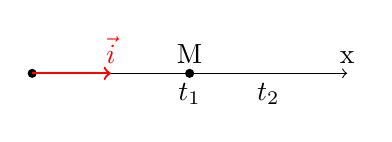
\begin{tikzpicture}
	\draw[->] (0, 0) -- (4, 0) node [above] {x};
	\draw[fill=black] (0,0) circle (0.05);
	\draw[fill=black] (2, 0) circle (0.05) node [above] {M} node [below] {$t_1$};
	\node[below] at (3, 0) {$t_2$};
	\draw[red, ->, thick] (0, 0) -- (1, 0) node [above] {$\vec{i}$};
\end{tikzpicture}

M se déplace sur $ox, (o, \vec{i})$ On repère M par $\overrightarrow{OM} = x\vec{i}$ avec x l'abscisse de M et $\overrightarrow{OM}$ le vecteur position.

En général, M dépend de t : \fbox{$\overrightarrow{OM}(t) = x(t)\vec{i}$}

\section{La vitesse}

La vitesse moyenne entre $t_1$ et $t_2$ : $<\vec{v}>_{[t_1, t_2]}= \frac{x(t_2)\vec{i} - x(t_1)\vec{i}}{t_2-t_1}$

$t_2=t_1+\Delta t \downarrow  \begin{array}{rcl} <\vec{v}> &=& \frac{x(t_2) - x(t_1)}{\Delta t} \vec{i} \\
<\vec{v}>_{\Delta t} &=& \frac{dM}{\Delta t} \vec{i} \text{Distance parcourue pendant} \Delta t \\
&=& \frac{\Delta x}{\Delta t}\vec{i}
\end{array}$

\section{Vitesse instantanée}

$v(t) = \lim_{\substack{t_2 \to t_1 \\ \Delta t \to 0}} \frac{x(t_2) - x(t_1)}{t_2 - t_1}\vec{i}$
	Ce qui donne $v(t) = \frac{dx}{dt}$ (dérivée de x par rapport à t).

	On note la dérivée $/_t$ : \fbox{$\dot{x}(t) = \frac{dx}{dt}=v(t)$}

\section{Accélération} : variation de $\vec{v}$ sur $[t_1, t_2]$ ~\\
	$\vec{a} = \frac{d\vec{v}}{dt} = \frac{dv(t)}{dt}\vec{i} = \dot{v}\vec{i}$

	or $ \begin{array}{rcl} v(t) &=& \frac{dx}{dt} \\
	a = \frac{d}{dt}(\frac{dx}{dt})=\frac{d^2x}{dt^2}
\end{array}$

donc \fbox{$\vec{a}=\dot{v}\vec{i} = \ddot{x}\vec{i}$}

\section{En 2D ou 3D} 

\begin{wrapfigure}[6]{l}{0pt}
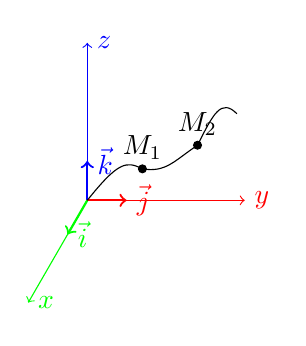
\begin{tikzpicture}
	\draw[->, red] (0, 0) -- (2, 0) node [right] {$y$};
	\draw[->, blue] (0, 0) -- (0, 2) node [right] {$z$};
	\draw[->, green] (0, 0) -- (-120:1.5) node [right] {$x$};

	\draw[->, thick, red] (0, 0) -- (0.5, 0) node [right] {$\vec{j}$};
	\draw[->, thick, blue] (0, 0) -- (0, 0.5) node [right] {$\vec{k}$};
	\draw[->, thick, green] (0, 0) -- (-120:0.5) node [right] {$\vec{i}$};
	\draw[] (0, 0) .. controls (0.4, 0.5) and (0.5, 0.5) .. (0.7, 0.4)  node [above] {$M_1$};
	\draw[] (0.7, 0.4) .. controls (1, 0.35) and (1.1, 0.5) .. (1.4, 0.7)node [above] {$M_2$};
	\draw[] (1.4, 0.7) .. controls (1.6, 1.1) and (1.7, 1.3) .. (1.9, 1.1);
	\draw[fill=black] (0.7, 0.4) circle (0.05);
	\draw[fill=black] (1.4, 0.7) circle (0.05);
\end{tikzpicture}
\end{wrapfigure}

La trajectoire est une courbe en 3D. M repéré par (x, y, z) dans la base orthonormée (o, $\vec{i}$, $\vec{j}$, $\vec{k}$).

$\overrightarrow{OM}(t) = x(t)\vec{i} + y(t)\vec{j} + z(t) \vec{k}$

Le vecteur vitesse : \[
	\begin{array}{rcl}
		<\vec{v}(t)_{[t_1, t_2]}> &=& \frac{\overrightarrow{OM}(t_2) - \overrightarrow{OM}(t_1)}{t_2-t_1} \\
		\vec{v}(t) &=& \frac{d(\overrightarrow{OM}_2-\overrightarrow{OM}_1}{dt} \\
										   &=& \frac{d}{dt}[(x_2\vec{i}+y_2\vec{j}+z_2{k})-(x_1\vec{i}+y_1\vec{j}+z_1{k}) \\
										   &=&\frac{dx}{dt}\vec{i} + \frac{dy}{dt}\vec{j}+\frac{dz}{dt}\vec{k} \\
										   &=& \dot{x}\vec{i}+\dot{y}\vec{j}+\dot{z}\vec{k}
\end{array}\]

\section{vecteur accélération} : 

$<\vec{a}>_{[t_1, t_2]} = \frac{\vec{v}(t_2)-\vec{v}(t_1)}{t_2-t_1}$ pour tout $t_2-t_1 = \Delta t \to \delta t$

\[\begin{array}{rcl}
	\vec{a} &=& \lim_{\Delta t \to 0} \frac{\Delta \vec{v}}{\Delta t} \\
		\vec{v}(t) &=& v_x\vec{i}+v_y\vec{j} + v_z\vec{k} \\
		\vec{a} &=& \frac{dv_x}{dt}\vec{i}+\frac{dv_y}{dt}\vec{j}+\frac{dv_z}{dt}\vec{k} \\
		&=& \frac{d^2x}{dt^2}\vec{i}+\frac{d^2y}{dt^2}\vec{j}+\frac{d^2z}{dt^2}\vec{k} 
\end{array}\]

\section{Dynamique du point matériel}

C'est l'étude des applications d'une force ou d'une action qui va modifier les mouvements des points matériels.
\section{1ere loi de Newton (1686-87): matériels}

\paragraph{1ère loi} Tout corps matériel persévère à l'état de repos ou de mouvement rectiligne dans lequel il se trouve à moins qu'une force quelconque n'agisse sur lui et le contraigne à changer d'état.

Les actions extérieures (Forces) changent l'état du système.

\begin{description}
	\item[Force] action dynamique qui va changer \ul{l'etat} du système \ul{physique}
\end{description}

\section{2eme loi de Newton}
\paragraph{énoncé} Le changement de mouvement d'un système se fait proportionnellement à l'action qui le provoque et dans le sens de celle ci.
La force change la \ul{quantite de mouvement} : proportionnelle à $\vec{v}$ et le facteur de proportionnalité m : \ul{masse}.

On note $\vec{P}=m\vec{v}$ la quantité de mouvement.

\fbox{$\frac{d\vec{P}}{dt}=\sum\vec{F}_{ext}$} ~\\
$\frac{d(m\vec{v})}{dt}=\sum\vec{F}_{ext}$ ~\\
$\frac{dm}{dt}\vec{v}+m\frac{d\vec{v}}{dt}=\sum\vec{F}_{ext}$

pour des masses constantes : $\left\{ \begin{array}{rcl}
		m\vec{a} &=& \sum\vec{F}_{ext} \\
		m\frac{d\vec{v}}{dt}&=&\sum\vec{F}_{ext}
	\end{array}\right\} $ = Principe Fondamentale de la Dynamique.

	\paragraph{En général} $\vec{F}$ dépend du temps et/ou de la position et/ou de la vitesse ~\\
	\fbox{$\vec{F}(\vec{OM}, \vec{v}) = m\frac{d\overrightarrow{OM}}{dt^2}$} relation entre les \ul{coordonees} et leurs dérivées : c'est une équation différentielle.

	\paragraph{Rappel} \[\begin{array}{rcl}
			{[F]} &=& MLT^{-2} \\
			{[\overrightarrow{v}]} &=& LT^{-1} \\
			{[\overrightarrow{a}]} &=& LT^{-2}
	\end{array}\]

	\section{Résolution d'un problème de dynamique}

	\begin{enumerate}
		\item \ul{identifier le systeme} et repérer les \ul{points} dont on veut étudier le comportement
		\item faire le bilan des force qui agissent en \ul{ce point} $\downarrow$ prodire le comportement des points en applicant le principe fondamentale de la dynamique : $\sum\vec{F}=m\vec{a}$
		\item définit la base orthonormé qui permet de "simplifier".
		\item on somme les forces et on les projette sur la base.
	\end{enumerate}

	\[\begin{array}{rcl}
			\vec{F}&=&F_x\vec{i}+F_y\vec{j}+F_z\vec{k} \\
			F_x&=&(x, y, z, \dot{x}, \dot{y}, \dot{z}, t) = m\dot{x} \\
			F_x&=&(x, y, z, \dot{x}, \dot{y}, \dot{z}, t) = m\dot{y} \\
			F_x&=&(x, y, z, \dot{x}, \dot{y}, \dot{z}, t) = m\dot{z}
	\end{array}\]
	Solution des Equations différentielles.
